\documentclass{article}

\usepackage{biblatex}
\addbibresource{../resources.bib}

\usepackage{graphicx}
\usepackage{tikz}
\usetikzlibrary{arrows}
\usetikzlibrary{quantikz}

\usepackage{physics}
\usepackage{amsthm}

\newtheorem{defn}{Definition}
\newtheorem{thrm}{Theorem}
\newtheorem{prob}{Problem}
\def\F{\mathcal{F}}

\title{Project Progress Report}
\author{Seyed Sajad Kahani \\ 22222815}

\begin{document}
\maketitle

\nocite{*}

\section{Literature Review}

\subsection{General Quantum Compilers}

\printbibliography[heading=none,keyword=general]

\subsection{Hamiltonian Quantum Compilers}

\printbibliography[heading=none,keyword=hamiltonian]

\subsection{Classical Problems in Compilation and Resource Allocation}

\printbibliography[heading=none,keyword=classical]

\section{The Aim}

To design and implement a problem-specific container, based on 2QAN, to be 

\begin{itemize}
    \item designed to use, not just a research project.
    \item made upon all previous efforts rather than just sticking to an specific idea.
    \item implemented based on the principles of compiler design.
\end{itemize}

\section{Results}

\subsection{Bridge Gate}

For a simple case, that we have three qubits, called $a, b, c$, and we want to apply a CNOT gate on $(a, c)$, but the connectivity only allows us to apply a CNOT gate on $(a, b)$ and $(b, c)$, the first solution would be to use a SWAP gate, which is shown in figure \ref{fig:bridge-one-with-swap} (7 gates, depth of 7)
  While another approach is to use a bridge gate, which is shown in figure \ref{fig:bridge-one-with-bridge} (4 gates, depth of 4).

  \def\qceq{\midstick[3,brackets=none]{=}}
  \begin{figure}[h]
    \label{fig:bridge-one-with-swap}
    \centering
    \begin{quantikz}
    \lstick{a} & \ctrl{2} & \qw \qceq & \swap{1} & \qw & \swap{1} & \qw\qceq & \ctrl{1} & \targ{} & \ctrl{1} & \qw &\ctrl{1} & \targ{} & \ctrl{1} & \qw \\
    \lstick{b} & \qw & \qw & \swap{} & \ctrl{1} & \swap{} & \qw & \targ{} & \ctrl{-1}& \targ{} & \ctrl{1} & \targ{} & \ctrl{-1}& \targ{} & \qw \\
    \lstick{c} & \targ{} & \qw  & \qw & \targ{} & \qw & \qw & \qw & \qw & \qw & \targ & \qw & \qw & \qw & \qw  & \qw \\
    \end{quantikz}
    \caption{Applying a CNOT gate on $(a, c)$ using a SWAP gate}
  \end{figure}

  \begin{figure}[h]
    \label{fig:bridge-one-with-bridge}
    \centering
    \begin{quantikz}
    \lstick{a} & \ctrl{2} & \qw \qceq & \qw & \ctrl{1} & \qw & \ctrl{1} & \qw \\
    \lstick{b} & \qw & \qw & \ctrl{1} & \targ{} & \ctrl{1}  & \targ{} & \qw \\
    \lstick{c} & \targ{} & \qw & \targ{} & \qw  & \targ & \qw  & \qw &  \qw \\
    \end{quantikz}
    \caption{Applying a CNOT gate on $(a, c)$ using a bridge gate}
  \end{figure}
  
  This example, could be generalized and the bridge gate must be generalized as well. Hereby we define the generalized version of the bridge gate and we show the optimality of the bridge gate in terms of the number of CNOT gates and the depth of the circuit.

  \def\qceq{\midstick[6,brackets=none]{=}}
  \begin{defn}{Generalized Bridge Gate}
    For an even $n$
    \begin{align*} \mathrm{Bridge}(1, n) = &\prod_{i=1}^{n/2 - 1}\mathrm{CNOT}(i + 1, i)\mathrm{CNOT}(n - i + 1, n - i) \\ & \prod_{i=1}^{n/2 - 1}\mathrm{CNOT}(i, i + 1)\mathrm{CNOT}(n - i, n - i + 1) \\ & \mathrm{Bridge}(n/2 - 1, n/2)  \\
    & \qty(\prod_{i=1}^{n/2 - 1}\mathrm{CNOT}(i + 1, i)\mathrm{CNOT}(n - i + 1, n - i))^\dagger \\ 
    & \qty(\prod_{i=1}^{n/2 - 1}\mathrm{CNOT}(i, i + 1)\mathrm{CNOT}(n - i, n - i + 1))^\dagger
    \end{align*}
    but for an odd $n$, it is a little bit different.
  \end{defn}

  \begin{figure}[h]
    \centering
\begin{quantikz}
\qw &\ctrl{5}&\qw\qceq&\targ{}  & \qw     &\ctrl{1}& \qw    & \qw    & \qw    &\ctrl{1}& \qw     &\targ{}&\qw\\
\qw & \qw    & \qw    &\ctrl{-1}&\targ{}  & \targ{}&\ctrl{1}& \qw    &\ctrl{1}&\targ{} &\targ{}  &\ctrl{-1}&\qw\\
\qw & \qw    & \qw    & \qw     &\ctrl{-1}& \qw    & \targ{}&\ctrl{1}&\targ{} & \qw    &\ctrl{-1}&\qw & \qw \\
\qw & \qw    & \qw    & \qw     &\targ{}  & \qw    &\ctrl{1}& \targ{}&\ctrl{1}& \qw    &\targ{}  &\qw & \qw\\
\qw & \qw    & \qw    &\targ{}  &\ctrl{-1}&\ctrl{1}& \targ{}& \qw    &\targ{} &\ctrl{1}&\ctrl{-1}&\targ{}&\qw \\
\qw &\targ{} & \qw    &\ctrl{-1}& \qw     & \targ{}& \qw    & \qw    & \qw    &\targ{} & \qw     &\ctrl{-1}& \qw 
\end{quantikz}
    \caption{The bridge gate for $n=6$}
  \end{figure}

  \begin{thrm}
    Assume that we decomposed a CNOT between the first and the last qubits in a chain, in terms of local circuit.
    This circuit must carry information from the first bit to the last and reverse.
    For the forward information flow, the information is an $X$ gate placed on the first qubit, will travel along the circuit, so we need to have a consequential $n$ CNOT gates to carry this information. The same argument is valid for a backward series of gates.
    Ignoring the first and the last qubit, for each qubit this argument is also valid that, the gate in those series must not be the first neither the last CNOT gate applied on the qubit.
    Therefore, at least we need to have two series, each has to have a range of CNOT gates, before and after.
    One could easily manage to find out that the simplest structure would be similar (in terms of complexity) to the proposed bridge gate.
  \end{thrm}


  As far as we know, the family of bridge gates with more than one qubit in the chain is not studied yet, and neither implemented in any quantum compiler. 
  It can be easily shown that for a simple case like the one in the figure \ref{fig:bridge-simplification} that we need to swap and return the qubits, using bridge gate can reduce both depth and number of gates. 

  \begin{figure}
    a) \\
    \begin{center}
    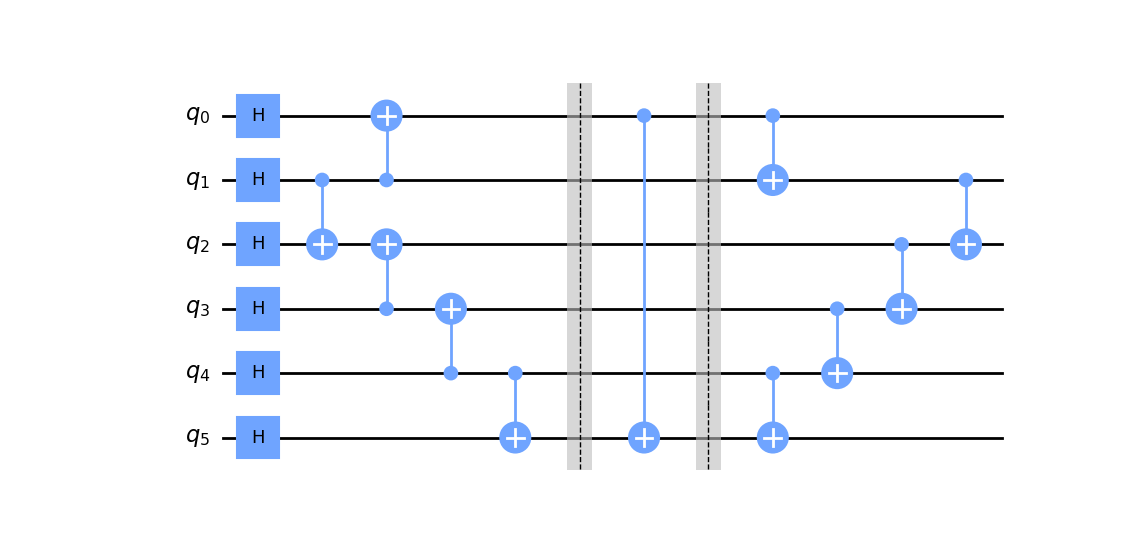
\includegraphics[width=0.9\textwidth]{../../code/expm_1_bridge/out/original_circuit}
    \end{center}
    b) \\
    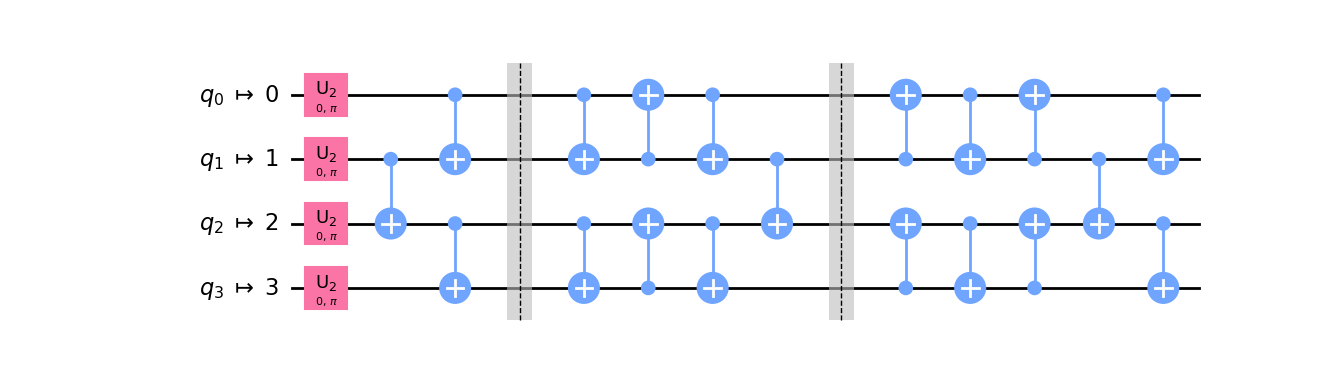
\includegraphics[width=0.9\textwidth]{../../code/expm_1_bridge/out/transpiled_circuit_swap} \\
    c) \\
    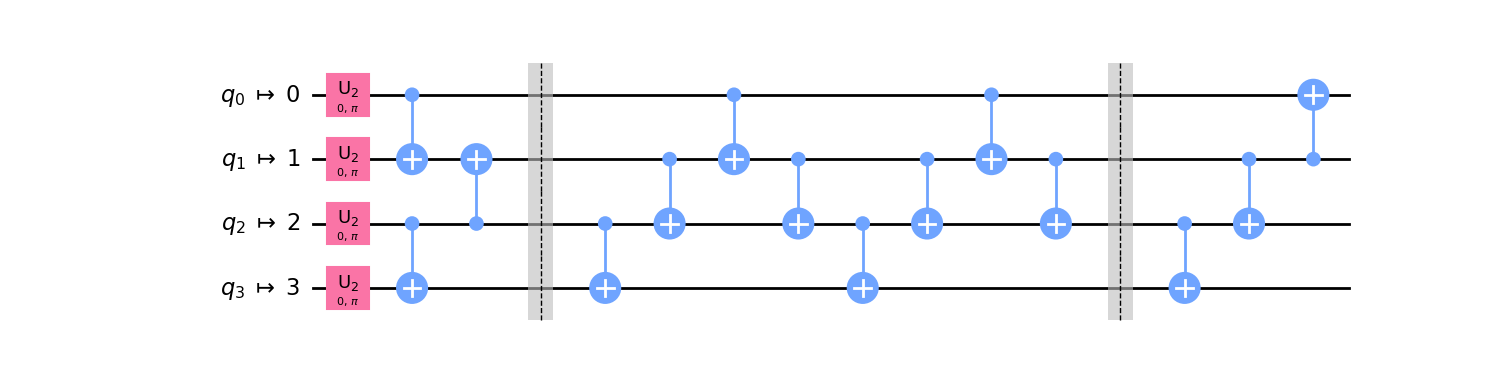
\includegraphics[width=0.9\textwidth]{../../code/expm_1_bridge/out/transpiled_circuit_bridge}
    \caption{a) The original circuit, consisting of some local operations, then a far away CNOT and then some local operations. b) The circuit after transpiling using Qiskit. c) The circuit after transpiling using bridge gate as an intermediate gate.}
  \end{figure}

\section{Challenges}

\begin{itemize}
\item Interdisciplinary work, a wide range of keywords, a wide range of languages in the papers.

\item The subtle line between theoretical works and applicability
\end{itemize}


\end{document}